% This document will contain some of the preliminary research and findings that I've been working on.
%
%
%
\documentclass{article}
\usepackage{amsmath}
\usepackage{graphicx}
\graphicspath{Images and Figures}

\title{Maritime Cybersecurity}
\author{William Smith}

\begin{document}
\maketitle
\begin{abstract}
%always write abstract last!    
\end{abstract}


\section{Introduction}
“Maritime Cyber Security Analysis – How to Reduce Threats?” names the following five areas susceptible to cyber attacks: Navigation Bridge, Power Management Systems, Engine Room, Cargo Handling Equipment, and Administrative and Communicational Systems[1]. This report looks to analyze each of the areas and highlight possible areas of vulnerability for attack. This report will also include a comprehensive analysis on the different  communication standards that are used to connect devices within an on-board ship network, as well as providing some context to the architecture of shipboard networks. Finally, recommendations will be made on different methods of modelling and testing the findings covered in this report.

\section{AIS}
Automated Information System (AIS) is a system that provides traffic monitoring, collision avoidance, aids to navigation, and more. AIS an important tool that is installed on hundreds of thousands of marine vessels worldwide, and is a mandatory requirement for vessels carrying more than a specified amount of cargo and passenger ships. While AIS has proven to be a very notable innovation in the automated maritime industry, it has a number of known exploits than range in severity. when a conversation about marine cybersecurity is initiated, AIS is a frequently noted offender [2]. 

AIS vulnerability overview here:
- these are not hard to find, lots of examples of people spoofing locations and hacking AIS...


\section{ECDIS}

Electronic Chart Display and Information System ECDIS is packaged as a software solution looking to directly replace paper nautical charts. ECDIS is installed on workstation PCs and was found to be primarily installed on machines running Windows XP. The ECDIS workstation pc acts as a point of convergence for other on-board systems and sensors. In recent years, the security of ECDIS systems have been called into question due to its inter-connectivity, leaving it vulnerable to specific cyber attacks and GPS spoofing. With the International Maritime Association (IMO) making the inclusion of ECDIS systems on board certain vessels mandatory, security and safety in the shipping and maritime industry has been of greater importance as of late. [4]. 


\section{NMEA}
The National Marine Electronics Association (NMEA) is a US based association that looks to create uniformity of electrical standards among manufacturers. This has been accomplished through the NMEA 0183 standard which has been widely accepted by manufacturers worldwide. NMEA 0183 has been available since 1983 and the newest version published in November 2018 continues to be widely used today. This standard uses the RS-422 electrical standard (most NMEA 0183 compatible devices also capable of driving a single RS-232 port) and uses an ASCII serial communications protocol that defines how data is transmitted by a single talker as sentences over a serial data bus for one or more listeners. NMEA is relatively slow, supporting a bandwidth of only 4800 bps and without the support for multiple talkers, it is not capable of creating networks. In leisure vessels, NMEA 0183 continues to be slowly phased out as the newer NMEA 2000 standard is replacing it, however, it continues to remain the go-to in commercial shipping applications.
[wiki and NMEA.org, ] 

NMEA 2000 is the newer, more sophisticated standard that is the successor to the NMEA 0183 standard. The purpose of NMEA 2000 is to create a single wire feed that acts as a backbone, with external devices and sensors connecting via a "Tee" connector piece, and a terminator connector on each end of the backbone. Another aspect in which NMEA differs is in how devices communicate with each other using this standard. NMEA 2000 compatible devices are connected using CAN (Controller Area Network) technology, and allows for the transmission and reception of data from multiple devices simultaneously. This makes it possible to implement integrated navigation and control systems solutions on board vessels of varying sizes. NMEA 2000 transmits data at a significantly higher rate than NMEA 0183 at speeds up to 250 kbps. It is common to find devices that process high volumes of information such as radar, electronic charts, and weather overlay information offer both Ethernet and NMEA 2000 connectivity. Where Ethernet is at a disadvantage is that there is no marine standard, making it not guaranteed that devices from different manufacturers are capable of communicating with each other. Ethernet also cannot prioritize the transmission of important information the same way NMEA 2000 can. Should multiple devices choose to communicate at the same time and a bus conflict occurs, with CAN, the device with the highest priority will go ahead with the transmission, and the lower priority device will try again later, where as with Ethernet the devices causing the collision will simply both stop transmitting and will try again later. This makes CAN a better suited solution for critical applications that require immediate response such as steering.
[7]   

\section{IEC 61162}
The International Electrotechnical Commission is the world leader in preparing and publishing international standards for a wide variety of electrical and electronic technologies. The IEC 61162 standards are a set of electrical communication standards strictly relating to "Digital interfaces for navigational equipment withing a ship". Each part of the IEC 61162 set of standards deal with the transport of NMEA sentences. a IEC 61162 includes NMEA 0183 in the form of IEC 61162-1, NMEA 2000 in the form of IEC 61162-3, and NMEA 0183 messages transported over IPv4 via Ethernet in the form of 61162-450, also known as Light Weight Ethernet (LWE) for its low protocol complexity. MORE ABOUT LWE.... LWE was developed with the intention of allowing efficient interfacing of equipment between manufacturers, as nearly all manufacturers simply have their own integrated bridge network solutions, which are typically based on Ethernet. LWE is intended to be used as an instrument or process layer network[5].

The last of the two standards defined by IEC 61162 are incremental upgrades in the form of a faster rate of data transmission for single talker and multiple listeners as IEC 61162-2, and a more secure add on to LWE as IEC 61162-460. There are very few implementations of IEC 61161-460 as it is a relatively new standard. [iec.ch and wiki] More information on each of these standards are available through IEC but require purchase.

\section{Navigation Bridge}
 
\section{Network layout}
Ships are made up of several complex interconnected systems, with each part complying with multiple industry standards depending on the manufacturer. Without a one size fits all solution for how layered ship networks are constructed, a general model can be assumed, and a number of manufacturers can be compared for differences and similarities in their network solutions. An example ship network architecture is one in which there are multiple layers, each of them connected to each other either through applications, generic firewalls, or gateway components.[5] 
\begin{figure}[h]
    \centering
    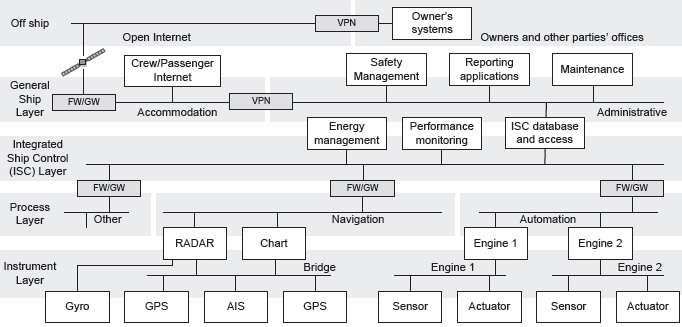
\includegraphics[width=12cm]{Images and Figures/isc-arch.jpg}
    \caption{Schematic Ship network Architecture [5]}
    \label{fig:network}
\end{figure}

The first of the five layers is the instrument layer, which is made up of several more simple devices and sensors that are connected to higher level components that use them. The lower level devices and sensors are typically connected to higher level systems using a serial communication protocol that depends on the system's manufacturer. 

With on-board ECDIS workstations being one of the main convergent points in the network of systems and sensors, ECDIS has been crucial part in understanding the network layouts on vessels using ECDIS solutions by common manufacturers. There are several different methods manufacturers are employing their networks, one of which is simply connecting the sensors directly to a main processing workstation, using the single talker, multiple listener IEC 61162-1/2 (NMEA 0183) standard, or other serial communications protocols like Modbus. Each of the ECDIS solutions offered by the Furuno, Transas, and Maris employ this method, where external devices and sensors such as AIS, GPS, Alarm Systems, and gyroscopes are connected directly to the processing unit, and additional sensors are connected to some a serial to LAN adaptor that is either connected directly to the processing unit or to a switching hub as shown below.
(Picture I've made of the network diagram for simple ecdis system)
[6][7]

\begin{figure}[h]
    \centering
    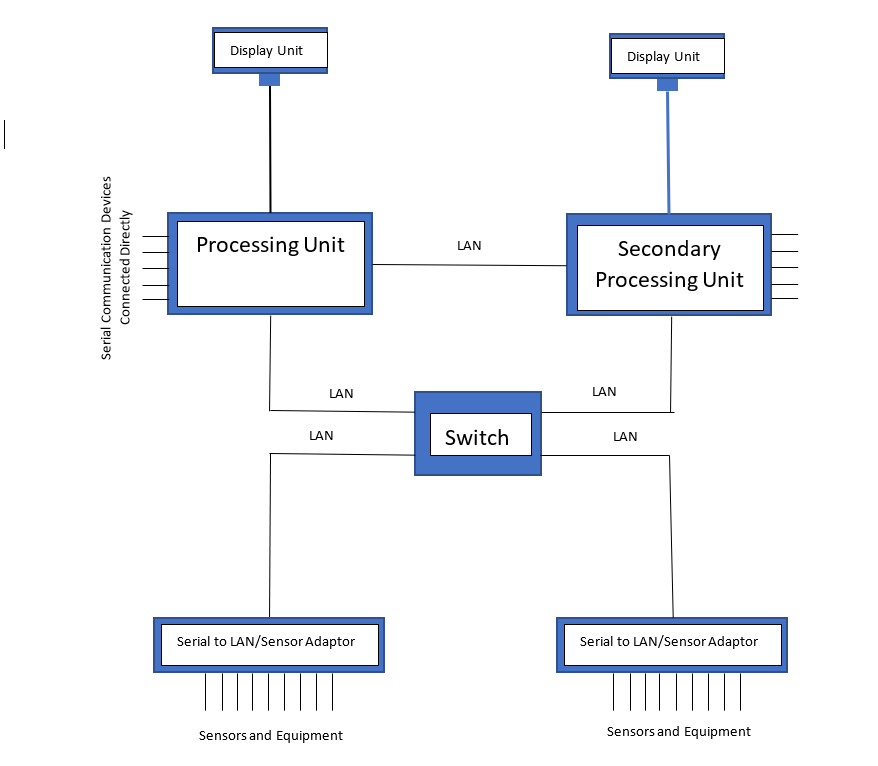
\includegraphics[width=12cm]{Images and Figures/ECDISsensorNetwork.PNG}
    \caption{ECDIS Sensor Network}
    \label{fig:network}
\end{figure}

An alternate configuration exists in which other manufacturers opt to use the NMEA-2000 communication standard, which allows devices to be connected directly to the backbone cable and and communicate over a CAN bus network. This network configuration is less frequently implemented in large shipping vessels, but is more widely used in smaller leisure vessels[5]. Simrad who offers ECDIS systems with smaller ships in mind, is a manufacturer whose solution follows this model.Simrad's wiring diagram is far simpler than that of the other previously mentioned manufacturers offering Ethernet and serial communication solution. Simrad's main workstation is connected to the backbone directly, along with any NMEA 2000 compatible sensors, the power supply, and terminator components on each end of the backbone. Maretron, a company that offers marine vessel monitoring and control systems solutions, offers a free NMEA 2000 network building software that allows you to design entire ship networks on the backbone of the NMEA 2000 standard. The following is an example of a 50ft sailboat that is offered through the software as an example network.

\begin{figure}[h]
    \centering
    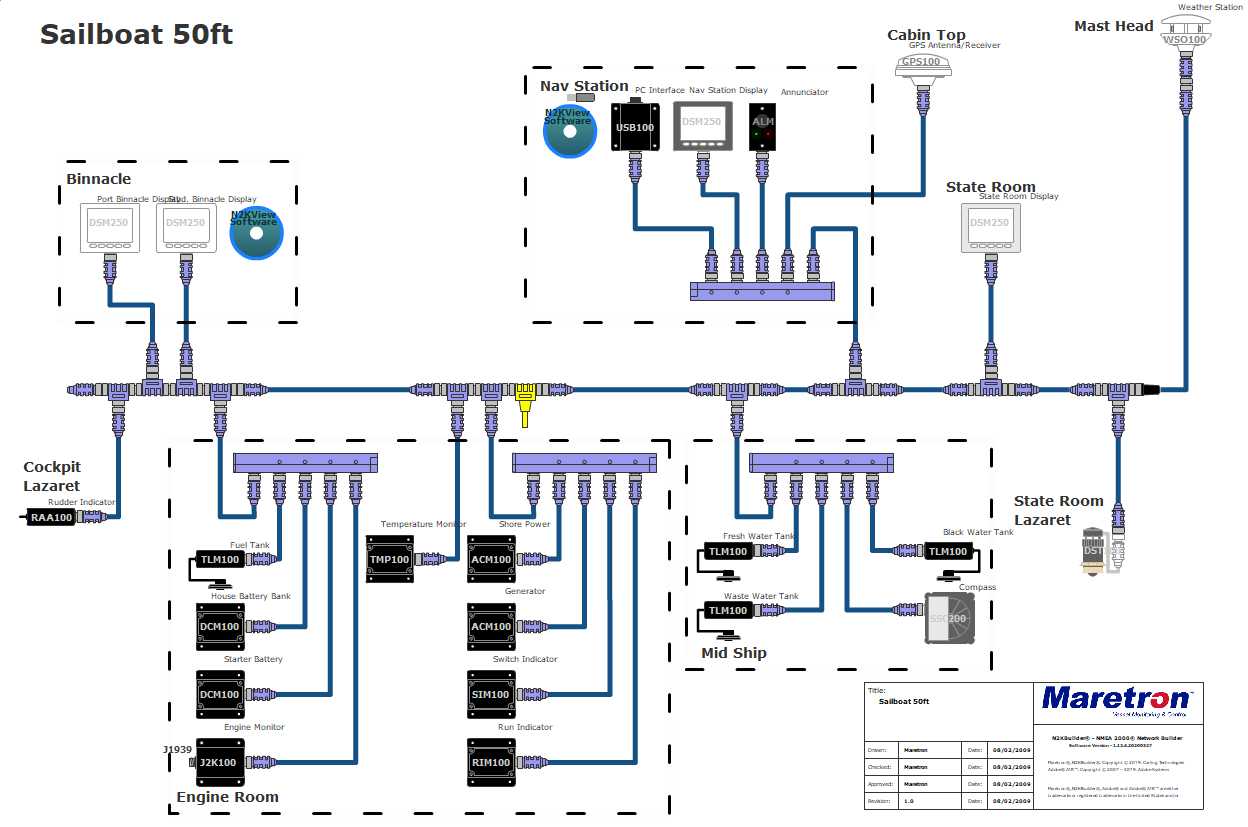
\includegraphics[width=12cm]{Images and Figures/NMEA2K.png}
    \caption{Example NMEA 2000 CAN on board 50ft sailboat   [5]}
    \label{fig:NMEA CAN}
\end{figure}




\section{Engine Room}
The engine room is an area on-board a vessel in which the engine and its accompanying components are housed. The company Maersk, A world-wide leader in overseas shipping is the owner of the biggest commercial cargo vessel, and will be the focus of the analysis in this section. Maersk vessels are powered by a diesel engine manufactured by Wärtsilä, and comes accompanied with the Wärtsilä Unified Control(UNIC) engine control system. This system is mounted locally on the engine in the form of a control panel and a display unit that shows operating data and an hour counter. The system has control over the engine's crucial operating functions such as its start/stop and  speed, as well as engine protection features such as alarms, shutdowns, and emergency stops. The controller uses the Modbus communication protocol to communicate with external systems either through Ethernet or serially[3]. 

\section{Creating a model}

Just some notes here.

using an arduino to simulate the ship, easy to interface with sensors and other serial communication devices. needs TTL to RS-485 adaptor 

Transas uses and optional PCI express 4xRS232 serial adaptor card that adds 4 serial ports to your system. this would be enough for a small subsystem of devices for testing. Transas also does a deeper dive into exactly the type of hardware it uses for its ecdis systems.

buying the NMEA 0183 standard is a little expensive, however much of it has been reverse engineered and is available for free online. This could be used in simple proof of concept tests.

\section{references}
put em here!

Mraković, I., \& Vojinović, R. (2019). Maritime cyber security analysis – How to reduce threats? Transactions on Maritime Science, 8(1), 132–139. https://doi.org/10.7225/toms.v08.n01.013 [1]

Balduzzi, M., Pasta, A., \& Wilhoit, K. (2014). A security evaluation of AIS automated identification system. ACM International Conference Proceeding Series, 2014-Decem(December), 436–445. https://doi.org/10.1145/2664243.2664257 [2]

Wärtsilä. (2016). Wärtsilä UNIC engine control system for diesel engines. 2. [3]

Dyryavyy, Y. (2015). Preparing for Cyber Battleships – Electronic Chart Display and Information System Security.[4]

Rødseth, Ø. J. (2006). Design challenges and decisions for a new ship data network. 450.[5]

Guide, I. (2009). NAVI-SAILOR.[6] fix this later - Installation manual for Transas' ECDIS product.

Krile, S., Kezić, D., \& Dimc, F. (2013). NMEA communication standard for shipboard data architecture | NMEA komunikacijski standard za arhitekturu podataka na brodu. Nase More, 60(3–4), 68–82. [7]


\end{document}


